\documentclass[aspectratio=169]{beamer}

\mode<presentation>

\usepackage[utf8]{inputenc}
\usepackage[T1]{fontenc}	%makes å,ä,ö etc. proper symbols
\usepackage{amsmath}
\usepackage{graphicx}
\usepackage{xcolor}
\usepackage{listings}
\usepackage{multicol}
\usepackage{hyperref}


\definecolor{LundaGroen}{RGB}{00,68,71}
\definecolor{StabilaLila}{RGB}{85,19,78}
\definecolor{VarmOrange}{RGB}{237,104,63}

\definecolor{MagnoliaRosa}{RGB}{251,214,209}
\definecolor{LundaHimmel}{RGB}{204,225,225}
\definecolor{LundaLjus}{RGB}{255,242,191}

\usefonttheme{serif}
\usetheme{malmoe}
\setbeamercolor{palette primary}{bg=VarmOrange}
\setbeamercolor{palette quaternary}{bg=LundaGroen}
\setbeamercolor{background canvas}{bg=LundaLjus}
\setbeamercolor{structure}{fg=LundaGroen}

\usepackage[many]{tcolorbox}

\newtcolorbox{cross}{blank,breakable,parbox=false,
  overlay={\draw[red,line width=5pt] (interior.south west)--(interior.north east);
    \draw[red,line width=5pt] (interior.north west)--(interior.south east);}}



\lstset{language=Python} 
\lstset{%language=[LaTeX]Tex,%C++,
    morekeywords={PassOptionsToPackage,selectlanguage,True,False},
    keywordstyle=\color{blue},%\bfseries,
    basicstyle=\small\ttfamily,
    %identifierstyle=\color{NavyBlue},
    commentstyle=\color{red}\ttfamily,
    stringstyle=\color{VarmOrange},
    numbers=left,%
    numberstyle=\scriptsize,%\tiny
    stepnumber=1,
    numbersep=8pt,
    showstringspaces=false,
    breaklines=true,
    %frameround=ftff,
    frame=single,
    belowcaptionskip=.75\baselineskip,
	tabsize=4,
	backgroundcolor=\color{white}
    %frame=L
}

\begin{document}

\lstset{literate=
  {á}{{\'a}}1 {é}{{\'e}}1 {í}{{\'i}}1 {ó}{{\'o}}1 {ú}{{\'u}}1
  {Á}{{\'A}}1 {É}{{\'E}}1 {Í}{{\'I}}1 {Ó}{{\'O}}1 {Ú}{{\'U}}1
  {à}{{\`a}}1 {è}{{\`e}}1 {ì}{{\`i}}1 {ò}{{\`o}}1 {ù}{{\`u}}1
  {À}{{\`A}}1 {È}{{\'E}}1 {Ì}{{\`I}}1 {Ò}{{\`O}}1 {Ù}{{\`U}}1
  {ä}{{\"a}}1 {ë}{{\"e}}1 {ï}{{\"i}}1 {ö}{{\"o}}1 {ü}{{\"u}}1
  {Ä}{{\"A}}1 {Ë}{{\"E}}1 {Ï}{{\"I}}1 {Ö}{{\"O}}1 {Ü}{{\"U}}1
  {â}{{\^a}}1 {ê}{{\^e}}1 {î}{{\^i}}1 {ô}{{\^o}}1 {û}{{\^u}}1
  {Â}{{\^A}}1 {Ê}{{\^E}}1 {Î}{{\^I}}1 {Ô}{{\^O}}1 {Û}{{\^U}}1
  {œ}{{\oe}}1 {Œ}{{\OE}}1 {æ}{{\ae}}1 {Æ}{{\AE}}1 {ß}{{\ss}}1
  {ű}{{\H{u}}}1 {Ű}{{\H{U}}}1 {ő}{{\H{o}}}1 {Ő}{{\H{O}}}1
  {ç}{{\c c}}1 {Ç}{{\c C}}1 {ø}{{\o}}1 {å}{{\r a}}1 {Å}{{\r A}}1
  {€}{{\euro}}1 {£}{{\pounds}}1 {«}{{\guillemotleft}}1
  {»}{{\guillemotright}}1 {ñ}{{\~n}}1 {Ñ}{{\~N}}1 {¿}{{?`}}1
}

\AtBeginSection[ ]
{
\begin{frame}{Outline}
    \tableofcontents[currentsection]
\end{frame}
}

\lstset{escapeinside={(*@}{@*)}}

\title{GUI med tkinter}
\date{vt 25}
\author{Programmering 2}

\maketitle

\section{Vad är ett GUI?}

\begin{frame}
\frametitle{Vad är ett GUI?}

GUI står för Graphical User Interface och betyder att du kan kommunicera med programmet utan att behöva använda dig utav konsolen som du har gjort tidigare.

Genom att använda ett GUI blir dina program användarvänligare.

\end{frame}

\section{tkinter}

\begin{frame}[fragile]
\frametitle{GUI med tkinter}

I Python är det vanligaste GUI-biblioteket \texttt{tkinter} som skapar ett fönster där du kan placera knappar, textfält och annat.

\begin{lstlisting}
import tkinter
\end{lstlisting}

\pause

I tidigare versioner av Python (före 3.0) så hette det Tkinter istället (notera stort T) så stöter du på äldre exempel så kan du oftast bara ändra till litet \texttt{t} så fungerar det mesta.

\end{frame}

\subsection{Skapa ett fönster}

\begin{frame}[fragile]
\frametitle{Skapa ett fönster i tkinter}

\begin{lstlisting}
import tkinter

root = tkinter.Tk()
\end{lstlisting}

\begin{figure}
	\begin{center}
	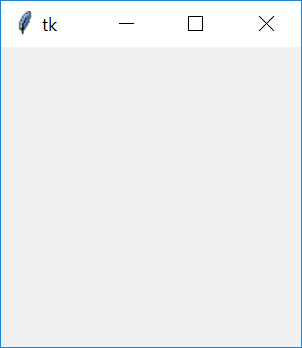
\includegraphics[width=0.2\textwidth]{win1.png}
	\caption{Ett tkinter-fönster}
	\end{center}
\end{figure}

\end{frame}

\subsection{Label}

\begin{frame}[fragile]
\frametitle{Text}

För att få ut text använder du widgeten \texttt{Label}

\begin{lstlisting}
import tkinter # Importera tkinter
root = tkinter.Tk() # Skapa fönstret

text = tkinter.Label(root, text='Kolla på mig')
text.pack() 
\end{lstlisting}

\begin{figure}
\begin{center}
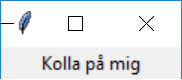
\includegraphics[]{win2.png}
\caption{Ett tkinter-fönster med text}
\end{center}
\end{figure}

\end{frame}

\begin{frame}[fragile]
\frametitle{Text}

\begin{lstlisting}
import tkinter # Importera tkinter
root = tkinter.Tk() # Skapa fönstret

tt = tkinter.Label(root, text='Kolla på mig')
tt.pack() 
\end{lstlisting}

Det första argumentet i \texttt{Label} är vilket fönster man ska koppla widgeten till. Sen kan man föra in ett par olika argument som man måste identifiera med deras \texttt{keywords}. \texttt{text} är då vad som ska skrivas.

Sen har alla widgetar en metod som kallas \texttt{pack()} som placerar ut objektet i fönstret.

\end{frame}

\subsection{Button}

\begin{frame}[fragile]
\frametitle{Knappar}

\begin{lstlisting}
import tkinter # Importera tkinter
root = tkinter.Tk() # Skapa fönstret
...
knapp = tkinter.Button(root, text="Click me", command=funk)
knapp.pack()
\end{lstlisting}

\begin{figure}
\begin{center}
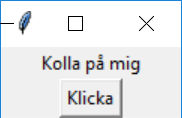
\includegraphics[]{win3.png}
\caption{Ett tkinter-fönster nu med en knapp}
\end{center}
\end{figure}

\end{frame}

\begin{frame}[fragile]
\frametitle{Knappar}

\begin{lstlisting}
text = tkinter.Label(root, text='Kolla på mig')
knapp = tkinter.Button(root, text="Click me", command=funk)
knapp.pack()
\end{lstlisting}

Jämför du \texttt{Label} med \texttt{Button} så ser du att skillnaden mellan en knapp och en label är att en knapp har en funktion kopplad till sig. Den funktionen behöver du skapa innan du skapar din knapp.

Det som är viktigt att notera med den här funktionen är att du ska bara skriva namnet i \texttt{command} och inte ha med paranteserna.

\end{frame}

\subsection{Entry}

\begin{frame}[fragile]
\frametitle{Användarinput}

\begin{lstlisting}
import tkinter # Importera tkinter
root = tkinter.Tk() # Skapa fönstret
...
fält = tkinter.Entry(root)
fält.pack()
\end{lstlisting}

\begin{figure}
\begin{center}
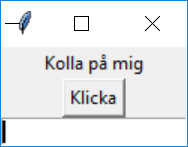
\includegraphics[]{win4.png}
\caption{Ett tkinter-fönster med ett input-fält}
\end{center}
\end{figure}

\end{frame}

\section{Läsa och ändra widgets}

\subsection{Läsa från widget}

\begin{frame}[fragile]
\frametitle{Läsa från fält}

\begin{lstlisting}
import tkinter
root = tkinter.Tk()
...
fält = tkinter.Entry(root)
fält.pack()

texten = fält.get()
\end{lstlisting}

\end{frame}

\begin{frame}[fragile]
\frametitle{Läsa från labels}

\begin{lstlisting}
import tkinter
root = tkinter.Tk()

tt = tkinter.Label(root, text='Kolla på mig')
tt.pack()

texten = tt.cget('text')
\end{lstlisting}

\end{frame}

\begin{frame}[fragile]
\frametitle{Läsa från annat än texten}

\begin{lstlisting}
import tkinter
root = tkinter.Tk()

tt = tkinter.Label(root, text='Kolla på mig', fg='red')
tt.pack()

var = tt.cget('fg')
\end{lstlisting}

\end{frame}

\subsection{Skriva till widget}

\begin{frame}[fragile]
\frametitle{Skriva till labels}

\begin{lstlisting}
import tkinter
root = tkinter.Tk()

tt = tkinter.Label(root, text='Kolla på mig')
tt.pack()

tt['text'] = 'Ny text'
\end{lstlisting}

Här kan du se att en widget typ fungerar som en dictionary, genom att ange vilket värde du vill ändra på i hakparanteserna så kan du ändra på texten och färgen.

\end{frame}

\section{Färger}

\begin{frame}[fragile]
\frametitle{Skriva till labels}

\begin{lstlisting}
import tkinter
root = tkinter.Tk()
tt = tkinter.Label(root, text='Kolla på mig', fg='yellow', bg='black')
tt.pack()
...
\end{lstlisting}

\begin{figure}
	\begin{center}
		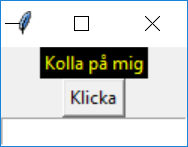
\includegraphics[width=0.15\textwidth]{win5.png}
		\caption{Nu har du bytt bakgrunds- och förgrundsfärg}
	\end{center}
\end{figure}

\end{frame}


\section{Övningar}

\begin{frame}
\frametitle{Övningar}

\begin{enumerate}
	\item Ladda ner filen \texttt{tkinter1.py} från Classroom och utgå från den.
	\item Lägg till två fält där man kan skriva
	\item Lägg till en knapp som med texten: ''+'' och skapa funktionen \texttt{add} som addererar talen i de båda fälten.
	\item Skriv ut resultatet i en \texttt{Label}.
	\item Lägg till knappar och funktioner för subtraktion, division och multiplikation.
\end{enumerate}
\end{frame}


\end{document}